\clearpage
\section{Exploratory integration of a trainable physiological core}
\label{app:physiology-pilot}

We additionally tested whether a language-model loss can train a physiological connectome module. This experiment is separate from the plastic-memory case studies in the main text. It establishes a trainable implementation, but does not establish useful memory performance or an advantage from biological connectivity.

\paragraph{Related implementations.}
FLM couples a fixed unsigned connectome reservoir to a frozen language backbone through a trained logit readout \citep{flm2026}. Fly as a Language Model describes trainable anatomical recurrent networks for text and location-question tasks \citep{flyaslm2026}. These precedents preclude a broad first-integration claim. Our pilot tests a distinct spiking construction; it does not establish superiority to either implementation.

\paragraph{Architecture.}
The input is a four-event history of objects moving between colored boxes. Each event is independently encoded using mean token embeddings from frozen Qwen3-4B and a trainable multilayer perceptron. The encoder supplies bounded currents to 128 olfactory input neurons in the full corrected graph of 138,639 neurons and 15,091,983 directed edges. The LIF dynamics use a 0.1-ms step, membrane and synaptic time constants of 20 and 5 ms, a 1.8-ms transmission delay, and a 2.2-ms refractory period. Four events of 128 steps each span 51.2 ms. The decoder maps final voltage and synaptic state at 384 output neurons to eight soft tokens. Qwen receives these tokens and the question, but no history text or history-bearing language-model cache.

The loss trains the encoder, decoder, and one positive presynaptic gain per neuron, constrained to $[0.25,2]$. Edge signs and topology are fixed. Threshold derivatives use a surrogate gradient; reset and refractory decisions are detached. Checkpointing carries the full delayed-signal queue and continuous state across temporal blocks. Online dopamine-gated plasticity is not used in this pilot: episode information resides in transient neural state, while gains are optimized across training examples.

\paragraph{Protocol.}
The generator produces 1,728 training, 288 validation, and 288 test examples. Each group contains two opposite orders of the target object's moves and two questions, with the same event multiset. Groups do not cross splits. Classes are balanced overall; words and event templates are shared across splits, so the test concerns held-out combinations rather than unrestricted language understanding. A fixed balanced subset of 48 validation examples selects checkpoints by first-answer-token negative log-likelihood. Both arms receive 1,000 batch-four updates, with 100 decoder-only warm-up updates followed by joint interface training and, in one arm, core training. Both selected checkpoints occur at update 400. The language model remains frozen. This is about 2.31 passes through the training set, with a single initialization.

\begin{table}[t]
\centering
\caption{Exploratory physiological-core language pilot. Accuracy (\%) on 288 held-out examples from 72 paired groups. A constant answer obtains 25\%; the last-mentioned-location heuristic obtains 62.5\%.}
\label{tab:physiology-pilot}
\begin{tabular}{lrrr}
\toprule
Variant & Normal & Zero state & State swap \\
\midrule
Trainable core & 28.82 & 25.00 & 27.43 \\
Frozen core & 23.96 & 23.61 & 26.39 \\
\bottomrule
\end{tabular}
\end{table}


\paragraph{Results and controls.}
The trainable and frozen cores obtain 28.82\% and 23.96\% test accuracy, respectively (Table~\ref{tab:physiology-pilot}). The paired-group bootstrap interval for their 4.86-percentage-point difference is $[-1.74,11.81]$ percentage points. The trainable variant's advantage over zero state is 3.82 points, with interval $[-2.08,9.38]$; its advantage over swapping the state with the opposite-order history is 1.39 points, with interval $[-1.74,4.86]$. These conditional intervals do not include initialization variability. Initial parameter hashes and data order match between arms, but their common warm-up phase is not bitwise reproducible; small differences therefore cannot be attributed solely to core training.

The selected trainable checkpoint changes 1,341 gains by more than $10^{-6}$, including 1,216 outside the input ports. This verifies parameter updates inside the graph, not useful learning. An earlier recipe collapsed the tested paired prefixes through input saturation. Revised clipping, learning rates, surrogate scale, batching, and warm-up preserve differences in all 12 inspected validation pairs, without establishing a reliable memory benefit. This is a combined recipe, not an isolated ablation.

\paragraph{Technical checks and diagnostic scope.}
After correcting refractory write semantics, a 300-ms matched-input replay agrees with Brian2 on the spike count of every neuron (26,175 spikes in total). This does not establish equality of all full-graph trajectories or biological validity. Seventeen local tests cover dynamics, delay handling, gradients, checkpoint equivalence, data grouping, and history exclusion from language-model inputs. A batch-four forward/backward profile uses about 10.2 GB of allocated memory on one 24-GB GPU and takes approximately 1.7 seconds per update.

The frozen language model solves 45 of 48 validation controls when supplied the original history as text. Separately, the same language decoder memorizes four fixed training states with a fixed question after 25 updates, generating all four correct words. This checks decoder trainability, not core learning or transfer. A numerical ridge probe on initial physiological states reaches 55.56\% on all 288 validation examples, with 95.14\% for the earlier object but 15.97\% for the last-mentioned object. An additional 12.8-ms settling period does not improve overall accuracy. These diagnostics leave conditional decoding, training exposure, and transfer to new combinations unresolved. No rewired-core or matched conventional recurrent-network comparison was performed.

\begin{figure}[t]
\centering
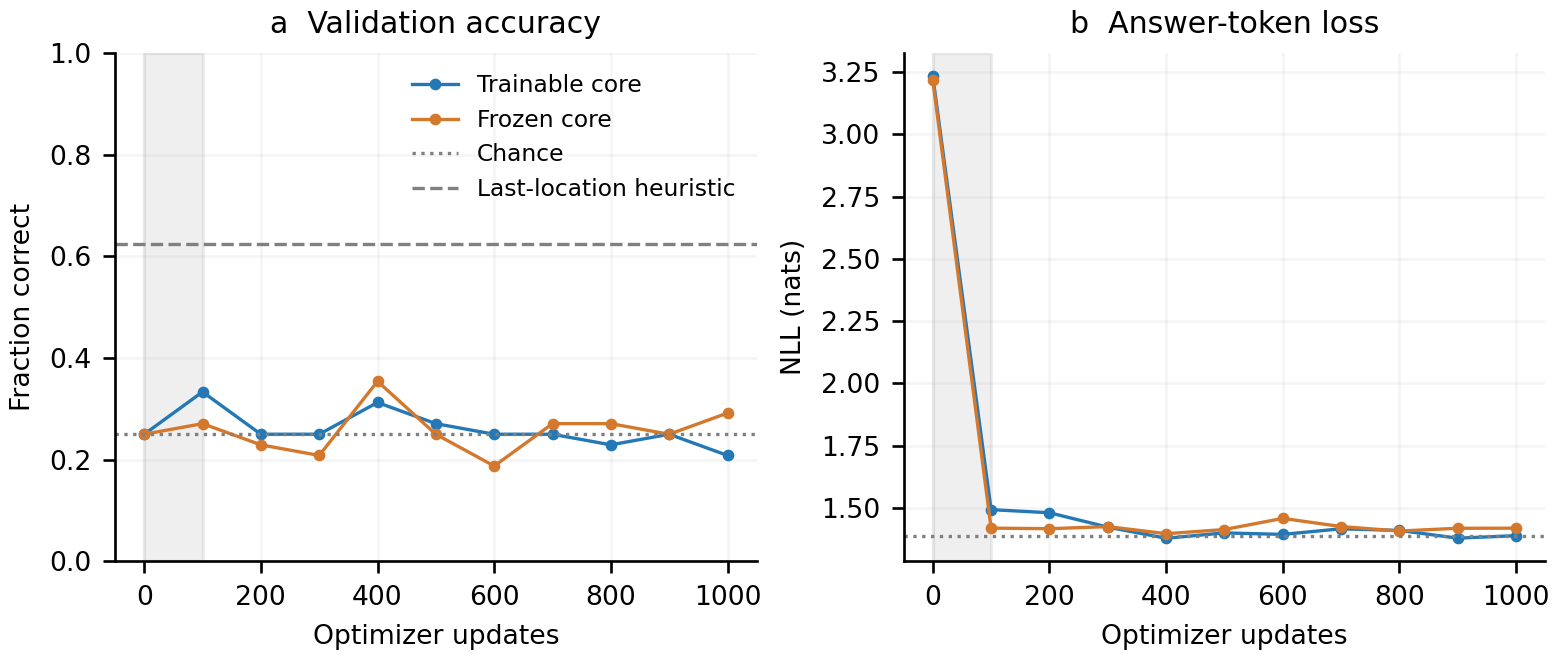
\includegraphics[width=\linewidth]{figures/physiology_hybrid_pilot.png}
\caption{Validation loss decreases toward a four-answer baseline, while accuracy remains low. Curves show the fixed 48-example validation subset; final test results are in Table~\ref{tab:physiology-pilot}. The shaded interval is decoder-only warm-up. Dotted accuracy lines denote 25\% chance performance; dashed lines denote the 62.5\% last-location heuristic. The dotted NLL line denotes a uniform distribution over four answers.}
\label{fig:physiology-pilot}
\end{figure}
